\documentclass[11pt,a4paper]{article}
\usepackage[margin=2.2cm]{geometry}
\usepackage{amsmath,amssymb,bm}
\usepackage{booktabs,multirow,array}
\usepackage[table]{xcolor}
\usepackage{pgfplots}
\pgfplotsset{compat=1.17}
\usetikzlibrary{patterns,calc}
\usepackage{listings}
\usepackage{float}
\usepackage{enumitem}
\usepackage{fancyhdr}
\usepackage[hidelinks]{hyperref}

\definecolor{headgray}{HTML}{E8E8E4}
\definecolor{pivot}{HTML}{F5C4B3}
\definecolor{feas}{HTML}{1D9E75}
\definecolor{objc}{HTML}{D85A30}
\definecolor{codebg}{HTML}{F7F7F4}

\lstset{basicstyle=\ttfamily\footnotesize,backgroundcolor=\color{codebg},frame=single,rulecolor=\color{black!25},
  breaklines=true,columns=fullflexible,keepspaces=true,showstringspaces=false,
  keywordstyle=\color{blue!60!black},commentstyle=\color{green!40!black},stringstyle=\color{red!55!black}}
\lstdefinestyle{out}{language={},backgroundcolor=\color{white},frame=leftline,rulecolor=\color{black!40}}

\pagestyle{fancy}\fancyhf{}
\lhead{MATH 303: Linear and Nonlinear Programming}\rhead{Assignment Solutions}\cfoot{\thepage}
\setlength{\parindent}{0pt}\setlength{\parskip}{6pt}

\newcommand{\answer}[1]{\begin{center}\fbox{\parbox{0.9\linewidth}{\centering\textbf{Answer:} #1}}\end{center}}

\title{\textbf{MATH 303: Linear and Nonlinear Programming}\\[4pt]\large Assignment Solutions: Graphical Method, Simplex Method and Python LP Solver}
\author{Mohammed Ayman\\ Zewail City of Science and Technology}
\date{November 2026}

\begin{document}
\maketitle

%=====================================================================
\section{Problem 1: Printed circuit boards (graphical method)}

\textbf{Formulation.} Let $x_1$ = number of boards of type $A$ and $x_2$ = number of boards of type $B$ produced per day.
\begin{align*}
\max\ & 10x_1+15x_2 \qquad\Longleftrightarrow\qquad \min f=-(10x_1+15x_2)\\
\text{s.t. } & 16x_1+10x_2\le 1500 &&\text{(component placement)}\\
& 10x_1+12x_2\le 1000 &&\text{(soldering)}\\
& 4x_1+8x_2\le 500 &&\text{(inspection)}\\
& x_1,\,x_2\ge 0
\end{align*}

\begin{figure}[H]\centering
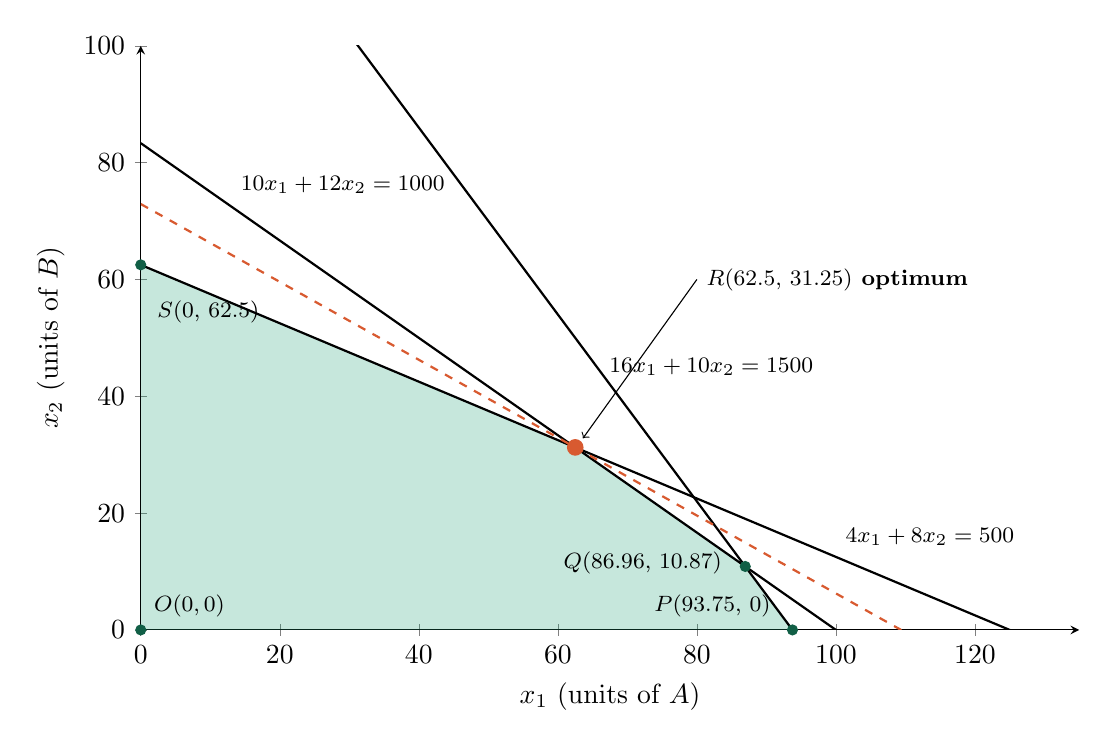
\begin{tikzpicture}
\begin{axis}[width=13.5cm,height=9cm,xmin=0,xmax=135,ymin=0,ymax=100,axis lines=left,
  xlabel={$x_1$ (units of $A$)},ylabel={$x_2$ (units of $B$)},xtick={0,20,...,120},ytick={0,20,...,100},clip=true]
\addplot[fill=feas,fill opacity=0.25,draw=none] coordinates {(0,0) (93.75,0) (86.957,10.870) (62.5,31.25) (0,62.5)} -- cycle;
\addplot[thick,domain=0:135,samples=2] {(1500-16*x)/10};
\addplot[thick,domain=0:135,samples=2] {(1000-10*x)/12};
\addplot[thick,domain=0:135,samples=2] {(500-4*x)/8};
\addplot[thick,dashed,objc,domain=0:135,samples=2] {(1093.75-10*x)/15};
\node[anchor=west,font=\footnotesize] at (axis cs:66,45) {$16x_1+10x_2=1500$};
\node[anchor=south west,font=\footnotesize] at (axis cs:13,73) {$10x_1+12x_2=1000$};
\node[anchor=west,font=\footnotesize] at (axis cs:100,16) {$4x_1+8x_2=500$};
\addplot[only marks,mark=*,mark size=1.8pt,feas!60!black] coordinates {(0,0) (93.75,0) (86.957,10.870) (0,62.5)};
\addplot[only marks,mark=*,mark size=2.8pt,objc] coordinates {(62.5,31.25)};
\node[anchor=south west,font=\footnotesize] at (axis cs:0.5,0.5) {$O(0,0)$};
\node[anchor=south east,font=\footnotesize] at (axis cs:92,0.5) {$P(93.75,\,0)$};
\node[anchor=east,font=\footnotesize] at (axis cs:85,11.5) {$Q(86.96,\,10.87)$};
\node[anchor=west,font=\footnotesize\bfseries] (Rl) at (axis cs:80,60) {$R(62.5,\,31.25)$ optimum};
\draw[->,thin] (Rl.west) -- (axis cs:63.6,32.8);
\node[anchor=north west,font=\footnotesize] at (axis cs:1,58) {$S(0,\,62.5)$};
\end{axis}
\end{tikzpicture}
\caption{Problem 1: feasible region (shaded) and the profit line through the optimum (dashed).}
\end{figure}

\textbf{Corner points.} $Q$ is the intersection of the placement and soldering lines; $R$ is the intersection of the soldering and inspection lines.
\begin{center}\renewcommand{\arraystretch}{1.2}
\begin{tabular}{clc}
\toprule
Point & $(x_1,\,x_2)$ & Profit $10x_1+15x_2$\\
\midrule
$O$ & $(0,\,0)$ & $0$\\
$P$ & $(93.75,\,0)$ & $937.5$\\
$Q$ & $(86.96,\,10.87)$ & $1032.61$\\
\rowcolor{pivot}$R$ & $(62.5,\,31.25)$ & $\mathbf{1093.75}$\\
$S$ & $(0,\,62.5)$ & $937.5$\\
\bottomrule
\end{tabular}\end{center}

\answer{$x_1^*=62.5$ boards of $A$, $x_2^*=31.25$ boards of $B$, maximum profit $=\$1093.75$ per day.}

Soldering and inspection times are fully used; $1500-16(62.5)-10(31.25)=187.5$ person-minutes of component-placement time remain unused.

\textbf{Python check.}
\begin{lstlisting}[language=Python]
"""
MATH 303 - Linear and Nonlinear Programming
Problem 1: PCB production (boards A and B)

    Max  f = 10 x1 + 15 x2            (x1 = units of A, x2 = units of B)
    s.t. 16 x1 + 10 x2 <= 1500        component placement
         10 x1 + 12 x2 <= 1000        soldering
          4 x1 +  8 x2 <=  500        inspection
         x1, x2 >= 0

linprog only minimizes, so we solve  Min f = -(10 x1 + 15 x2).
"""
from scipy.optimize import linprog

c = [-10, -15]                      # Min f = -(10 x1 + 15 x2)
A_ub = [[16, 10],
        [10, 12],
        [4, 8]]
b_ub = [1500, 1000, 500]
bounds = [(0, None), (0, None)]

res = linprog(c, A_ub=A_ub, b_ub=b_ub, bounds=bounds, method="highs")

print("Status :", res.message)
print(f"x1 (A) = {res.x[0]:.4f}")
print(f"x2 (B) = {res.x[1]:.4f}")
print(f"Max profit f = {-res.fun:.4f}")
print("Slacks (placement, soldering, inspection):", res.slack)
\end{lstlisting}
\begin{lstlisting}[style=out]
Status : Optimization terminated successfully. (HiGHS Status 7: Optimal)
x1 (A) = 62.5000
x2 (B) = 31.2500
Max profit f = 1093.7500
Slacks (placement, soldering, inspection): [187.5   0.    0. ]
\end{lstlisting}

%=====================================================================
\newpage
\section{Problem 2}
\begin{align*}
\max\ & x-8y\\
\text{s.t. } & 3x+2y\ge 6,\quad x-y\le 6,\quad 9x+7y\le 108,\quad 3x+7y\le 70,\quad 2x-5y\ge -35,\quad x,y\ge 0
\end{align*}

\subsection*{(a) Simplex method}
Let $x_1=x$, $x_2=y$. The last constraint is multiplied by $-1$ to make its right-hand side positive. With surplus $x_3$, slacks $x_4,\dots,x_7$ and artificial $x_8$:
\begin{align*}
\min f=\ & -x_1+8x_2+Mx_8\\
& 3x_1+2x_2-x_3+x_8=6\\
& x_1-x_2+x_4=6\\
& 9x_1+7x_2+x_5=108\\
& 3x_1+7x_2+x_6=70\\
& -2x_1+5x_2+x_7=35,\qquad x_1,\dots,x_8\ge 0
\end{align*}
Here $n=8$, $m=5$; the initial basic variables are $x_8,x_4,x_5,x_6,x_7$.

\begin{center}\renewcommand{\arraystretch}{1.35}\setlength{\tabcolsep}{4.5pt}\small
\begin{tabular}{|c|c|cccccccc|c|c|}
\hline
\rowcolor{headgray}\textbf{Iter.} & \textbf{Basic} & $x_{1}$ & $x_{2}$ & $x_{3}$ & $x_{4}$ & $x_{5}$ & $x_{6}$ & $x_{7}$ & $x_{8}$ & $b$ & \textbf{Ratio} \\ \hline
\multirow{6}{*}{0} & $x_{8}$ & \cellcolor{pivot}$\mathbf{3}$ & $2$ & $-1$ & $0$ & $0$ & $0$ & $0$ & $1$ & $6$ & $2$ $\leftarrow$ \\
 & $x_{4}$ & $1$ & $-1$ & $0$ & $1$ & $0$ & $0$ & $0$ & $0$ & $6$ & $6$ \\
 & $x_{5}$ & $9$ & $7$ & $0$ & $0$ & $1$ & $0$ & $0$ & $0$ & $108$ & $12$ \\
 & $x_{6}$ & $3$ & $7$ & $0$ & $0$ & $0$ & $1$ & $0$ & $0$ & $70$ & $\tfrac{70}{3}$ \\
 & $x_{7}$ & $-2$ & $5$ & $0$ & $0$ & $0$ & $0$ & $1$ & $0$ & $35$ &  \\
\cline{2-12}
 & $f$ & $-1-3M$ & $8-2M$ & $M$ & $0$ & $0$ & $0$ & $0$ & $0$ & $-f=-6M$ & $x_{1}$ in, $x_{8}$ out \\ \hline
\multirow{6}{*}{1} & $x_{1}$ & $1$ & $\tfrac{2}{3}$ & $-\tfrac{1}{3}$ & $0$ & $0$ & $0$ & $0$ & $\tfrac{1}{3}$ & $2$ &  \\
 & $x_{4}$ & $0$ & $-\tfrac{5}{3}$ & \cellcolor{pivot}$\mathbf{\tfrac{1}{3}}$ & $1$ & $0$ & $0$ & $0$ & $-\tfrac{1}{3}$ & $4$ & $12$ $\leftarrow$ \\
 & $x_{5}$ & $0$ & $1$ & $3$ & $0$ & $1$ & $0$ & $0$ & $-3$ & $90$ & $30$ \\
 & $x_{6}$ & $0$ & $5$ & $1$ & $0$ & $0$ & $1$ & $0$ & $-1$ & $64$ & $64$ \\
 & $x_{7}$ & $0$ & $\tfrac{19}{3}$ & $-\tfrac{2}{3}$ & $0$ & $0$ & $0$ & $1$ & $\tfrac{2}{3}$ & $39$ &  \\
\cline{2-12}
 & $f$ & $0$ & $\tfrac{26}{3}$ & $-\tfrac{1}{3}$ & $0$ & $0$ & $0$ & $0$ & $\tfrac{1}{3}+M$ & $-f=2$ & $x_{3}$ in, $x_{4}$ out \\ \hline
\multirow{6}{*}{2} & $x_{1}$ & $1$ & $-1$ & $0$ & $1$ & $0$ & $0$ & $0$ & $0$ & $6$ &  \\
 & $x_{3}$ & $0$ & $-5$ & $1$ & $3$ & $0$ & $0$ & $0$ & $-1$ & $12$ &  \\
 & $x_{5}$ & $0$ & $16$ & $0$ & $-9$ & $1$ & $0$ & $0$ & $0$ & $54$ &  \\
 & $x_{6}$ & $0$ & $10$ & $0$ & $-3$ & $0$ & $1$ & $0$ & $0$ & $52$ &  \\
 & $x_{7}$ & $0$ & $3$ & $0$ & $2$ & $0$ & $0$ & $1$ & $0$ & $47$ &  \\
\cline{2-12}
 & $f$ & $0$ & $7$ & $0$ & $1$ & $0$ & $0$ & $0$ & $M$ & $-f=6$ & optimal \\ \hline
\end{tabular}\end{center}

Final basic solution: $x_1=6,\ x_3=12,\ x_5=54,\ x_6=52,\ x_7=47$; non-basic $x_2=x_4=x_8=0$; $\min f=-6$.

\answer{$x^*=6,\ y^*=0,\ \max f=6$.}

\subsection*{(b) Graphical method}
\begin{figure}[H]\centering
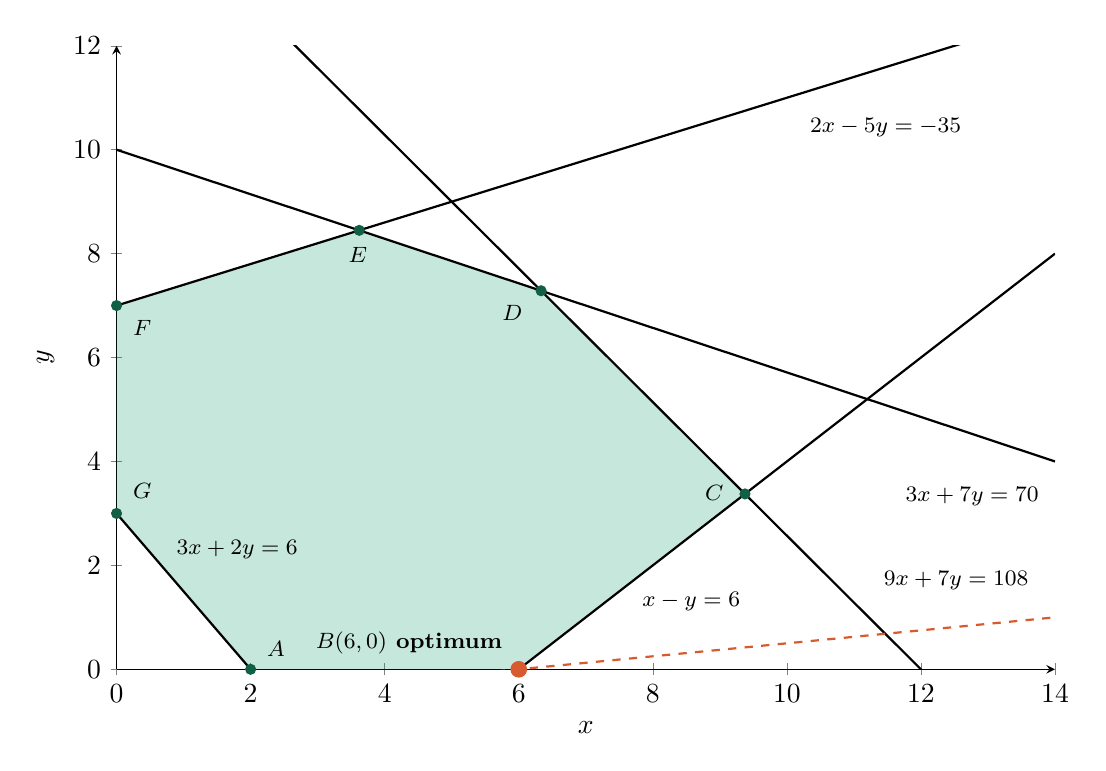
\begin{tikzpicture}
\begin{axis}[width=13.5cm,height=9.5cm,xmin=0,xmax=14,ymin=0,ymax=12,axis lines=left,xlabel={$x$},ylabel={$y$},xtick={0,2,...,14},ytick={0,2,...,12}]
\addplot[fill=feas,fill opacity=0.25,draw=none] coordinates {(2,0) (6,0) (9.375,3.375) (6.3333,7.2857) (3.6207,8.4483) (0,7) (0,3)} -- cycle;
\addplot[thick,domain=0:14,samples=2] {(6-3*x)/2};
\addplot[thick,domain=0:14,samples=2] {x-6};
\addplot[thick,domain=0:14,samples=2] {(108-9*x)/7};
\addplot[thick,domain=0:14,samples=2] {(70-3*x)/7};
\addplot[thick,domain=0:14,samples=2] {(2*x+35)/5};
\addplot[thick,dashed,objc,domain=0:14,samples=2] {(x-6)/8};
\node[anchor=west,font=\footnotesize] at (axis cs:0.75,2.3) {$3x+2y=6$};
\node[anchor=west,font=\footnotesize] at (axis cs:7.7,1.3) {$x-y=6$};
\node[anchor=west,font=\footnotesize] at (axis cs:11.3,1.7) {$9x+7y=108$};
\node[anchor=north east,font=\footnotesize] at (axis cs:13.9,3.7) {$3x+7y=70$};
\node[anchor=north west,font=\footnotesize] at (axis cs:10.2,10.8) {$2x-5y=-35$};
\addplot[only marks,mark=*,mark size=1.8pt,feas!60!black] coordinates {(2,0) (9.375,3.375) (6.3333,7.2857) (3.6207,8.4483) (0,7) (0,3)};
\addplot[only marks,mark=*,mark size=2.8pt,objc] coordinates {(6,0)};
\node[anchor=south west,font=\footnotesize] at (axis cs:2.1,0.05) {$A$};
\node[anchor=south east,font=\footnotesize\bfseries] at (axis cs:5.9,0.1) {$B(6,0)$ optimum};
\node[anchor=east,font=\footnotesize] at (axis cs:9.2,3.4) {$C$};
\node[anchor=north east,font=\footnotesize] at (axis cs:6.2,7.2) {$D$};
\node[anchor=north,font=\footnotesize] at (axis cs:3.6,8.3) {$E$};
\node[anchor=north west,font=\footnotesize] at (axis cs:0.1,6.9) {$F$};
\node[anchor=south west,font=\footnotesize] at (axis cs:0.1,3.1) {$G$};
\end{axis}
\end{tikzpicture}
\caption{Problem 2: feasible region and the objective line $x-8y=6$ through the optimum.}
\end{figure}

\begin{center}\renewcommand{\arraystretch}{1.25}
\begin{tabular}{cllc}
\toprule
Point & Intersection of & $(x,\,y)$ & $f=x-8y$\\
\midrule
$A$ & $3x+2y=6$, $y=0$ & $(2,\,0)$ & $2$\\
\rowcolor{pivot}$B$ & $x-y=6$, $y=0$ & $(6,\,0)$ & $\mathbf{6}$\\
$C$ & $x-y=6$, $9x+7y=108$ & $\left(\tfrac{75}{8},\,\tfrac{27}{8}\right)$ & $-17.625$\\
$D$ & $9x+7y=108$, $3x+7y=70$ & $\left(\tfrac{19}{3},\,\tfrac{51}{7}\right)$ & $-51.95$\\
$E$ & $3x+7y=70$, $2x-5y=-35$ & $\left(\tfrac{105}{29},\,\tfrac{245}{29}\right)$ & $-63.97$\\
$F$ & $2x-5y=-35$, $x=0$ & $(0,\,7)$ & $-56$\\
$G$ & $3x+2y=6$, $x=0$ & $(0,\,3)$ & $-24$\\
\bottomrule
\end{tabular}\end{center}
The largest value of $f$ occurs at $B(6,0)$, in agreement with the simplex result: $\max f=6$.

\subsection*{(c) Python LP solver}
\begin{lstlisting}[language=Python]
"""
MATH 303 - Linear and Nonlinear Programming
Problem 2

    Max  f = x - 8y
    s.t. 3x + 2y >= 6
          x -  y <= 6
         9x + 7y <= 108
         3x + 7y <= 70
         2x - 5y >= -35
         x, y >= 0

Converted for linprog (Min, all constraints as <=):
    Min f = -(x - 8y) = -x + 8y
    -3x - 2y <= -6
     -2x + 5y <= 35
"""
from scipy.optimize import linprog

c = [-1, 8]                         # Min f = -x + 8y
A_ub = [[-3, -2],                   # 3x + 2y >= 6
        [1, -1],
        [9, 7],
        [3, 7],
        [-2, 5]]                    # 2x - 5y >= -35
b_ub = [-6, 6, 108, 70, 35]
bounds = [(0, None), (0, None)]

res = linprog(c, A_ub=A_ub, b_ub=b_ub, bounds=bounds, method="highs")

print("Status :", res.message)
print(f"x = {res.x[0]:.4f}")
print(f"y = {res.x[1]:.4f}")
print(f"Max f = {-res.fun:.4f}")
\end{lstlisting}
\begin{lstlisting}[style=out]
Status : Optimization terminated successfully. (HiGHS Status 7: Optimal)
x = 6.0000
y = 0.0000
Max f = 6.0000
\end{lstlisting}

%=====================================================================
\newpage
\section{Problem 3}
\begin{align*}
\min f=\ & 2x_1+4x_2\\
\text{s.t. } & x_1+x_2\le 8,\qquad 6x_1+4x_2\ge 12,\qquad x_1+4x_2=20,\qquad x_1,x_2\ge 0
\end{align*}

\subsection*{(a) Simplex method (minimization)}
With slack $x_3$, surplus $x_4$ and artificials $x_5$ (second constraint) and $x_6$ (equality constraint):
\begin{align*}
\min f=\ & 2x_1+4x_2+Mx_5+Mx_6\\
& x_1+x_2+x_3=8\\
& 6x_1+4x_2-x_4+x_5=12\\
& x_1+4x_2+x_6=20,\qquad x_1,\dots,x_6\ge 0
\end{align*}
Here $n=6$, $m=3$; the initial basic variables are $x_3,x_5,x_6$.

\begin{center}\renewcommand{\arraystretch}{1.35}\setlength{\tabcolsep}{4.5pt}\small
\begin{tabular}{|c|c|cccccc|c|c|}
\hline
\rowcolor{headgray}\textbf{Iter.} & \textbf{Basic} & $x_{1}$ & $x_{2}$ & $x_{3}$ & $x_{4}$ & $x_{5}$ & $x_{6}$ & $b$ & \textbf{Ratio} \\ \hline
\multirow{4}{*}{0} & $x_{3}$ & $1$ & $1$ & $1$ & $0$ & $0$ & $0$ & $8$ & $8$ \\
 & $x_{5}$ & $6$ & \cellcolor{pivot}$\mathbf{4}$ & $0$ & $-1$ & $1$ & $0$ & $12$ & $3$ $\leftarrow$ \\
 & $x_{6}$ & $1$ & $4$ & $0$ & $0$ & $0$ & $1$ & $20$ & $5$ \\
\cline{2-10}
 & $f$ & $2-7M$ & $4-8M$ & $0$ & $M$ & $0$ & $0$ & $-f=-32M$ & $x_{2}$ in, $x_{5}$ out \\ \hline
\multirow{4}{*}{1} & $x_{3}$ & $-\tfrac{1}{2}$ & $0$ & $1$ & $\tfrac{1}{4}$ & $-\tfrac{1}{4}$ & $0$ & $5$ & $20$ \\
 & $x_{2}$ & $\tfrac{3}{2}$ & $1$ & $0$ & $-\tfrac{1}{4}$ & $\tfrac{1}{4}$ & $0$ & $3$ &  \\
 & $x_{6}$ & $-5$ & $0$ & $0$ & \cellcolor{pivot}$\mathbf{1}$ & $-1$ & $1$ & $8$ & $8$ $\leftarrow$ \\
\cline{2-10}
 & $f$ & $-4+5M$ & $0$ & $0$ & $1-M$ & $-1+2M$ & $0$ & $-f=-12-8M$ & $x_{4}$ in, $x_{6}$ out \\ \hline
\multirow{4}{*}{2} & $x_{3}$ & $\tfrac{3}{4}$ & $0$ & $1$ & $0$ & $0$ & $-\tfrac{1}{4}$ & $3$ &  \\
 & $x_{2}$ & $\tfrac{1}{4}$ & $1$ & $0$ & $0$ & $0$ & $\tfrac{1}{4}$ & $5$ &  \\
 & $x_{4}$ & $-5$ & $0$ & $0$ & $1$ & $-1$ & $1$ & $8$ &  \\
\cline{2-10}
 & $f$ & $1$ & $0$ & $0$ & $0$ & $M$ & $-1+M$ & $-f=-20$ & optimal \\ \hline
\end{tabular}\end{center}

Both artificial variables have left the basis, so the solution is feasible for the original problem.

\answer{$x_1^*=0,\ x_2^*=5,\ \min f=20$ \quad ($x_3=3,\ x_4=8$).}

\subsection*{(b) Graphical method}
Because of the equality constraint, the feasible region is not an area: it is the part of the line $x_1+4x_2=20$ that also satisfies the two inequalities and $x_1,x_2\ge0$. Substituting $x_1=20-4x_2$ in $x_1+x_2\le 8$ gives $x_2\ge 4$, and $x_1\ge 0$ gives $x_2\le 5$; the constraint $6x_1+4x_2\ge 12$ holds everywhere on this piece. The feasible set is therefore the segment joining $A(0,5)$ and $B(4,4)$.

\begin{figure}[H]\centering
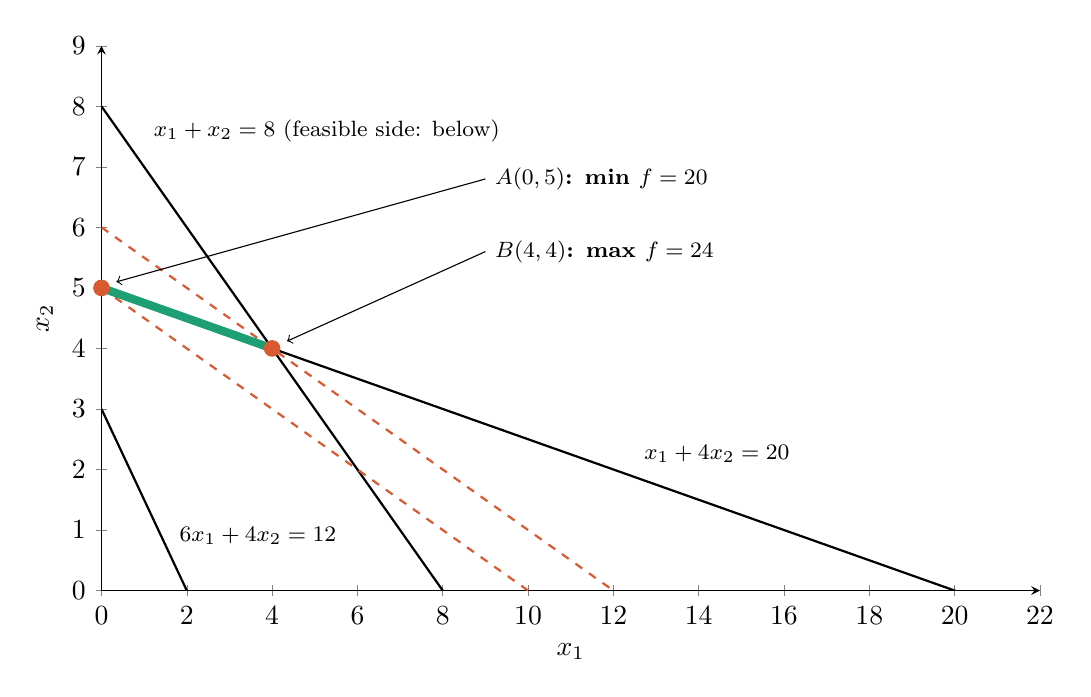
\begin{tikzpicture}
\begin{axis}[width=13.5cm,height=8.5cm,xmin=0,xmax=22,ymin=0,ymax=9,axis lines=left,xlabel={$x_1$},ylabel={$x_2$},xtick={0,2,...,22},ytick={0,1,...,9}]
\addplot[thick,domain=0:22,samples=2] {8-x};
\addplot[thick,domain=0:22,samples=2] {(12-6*x)/4};
\addplot[thick,domain=0:22,samples=2] {(20-x)/4};
\addplot[thick,dashed,objc,domain=0:22,samples=2] {(20-2*x)/4};
\addplot[thick,dashed,objc,domain=0:22,samples=2] {(24-2*x)/4};
\addplot[line width=3pt,feas] coordinates {(0,5) (4,4)};
\node[anchor=west,font=\footnotesize] at (axis cs:1.0,7.6) {$x_1+x_2=8$ (feasible side: below)};
\node[anchor=west,font=\footnotesize] at (axis cs:1.6,0.9) {$6x_1+4x_2=12$};
\node[anchor=south west,font=\footnotesize] at (axis cs:12.5,1.95) {$x_1+4x_2=20$};
\addplot[only marks,mark=*,mark size=2.8pt,objc] coordinates {(0,5) (4,4)};
\node[anchor=west,font=\footnotesize\bfseries] (Al) at (axis cs:9,6.8) {$A(0,5)$: min $f=20$};
\draw[->,thin] (Al.west) -- (axis cs:0.35,5.1);
\node[anchor=west,font=\footnotesize\bfseries] (Bl) at (axis cs:9,5.6) {$B(4,4)$: max $f=24$};
\draw[->,thin] (Bl.west) -- (axis cs:4.35,4.12);
\end{axis}
\end{tikzpicture}
\caption{Problem 3: the feasible set is the thick segment $AB$; the dashed lines are the objective contours $f=20$ (through $A$) and $f=24$ (through $B$).}
\end{figure}

\begin{center}\renewcommand{\arraystretch}{1.2}
\begin{tabular}{clc}
\toprule
Point & $(x_1,\,x_2)$ & $f=2x_1+4x_2$\\
\midrule
$A$ & $(0,\,5)$ & $20$ \ (minimum)\\
$B$ & $(4,\,4)$ & $24$ \ (maximum)\\
\bottomrule
\end{tabular}\end{center}

\subsection*{(d) Maximize $f=2x_1+4x_2$}
The constraints are unchanged; only the objective is converted: $\max(2x_1+4x_2)\equiv\min f=-2x_1-4x_2+Mx_5+Mx_6$.

\begin{center}\renewcommand{\arraystretch}{1.35}\setlength{\tabcolsep}{4.5pt}\small
\begin{tabular}{|c|c|cccccc|c|c|}
\hline
\rowcolor{headgray}\textbf{Iter.} & \textbf{Basic} & $x_{1}$ & $x_{2}$ & $x_{3}$ & $x_{4}$ & $x_{5}$ & $x_{6}$ & $b$ & \textbf{Ratio} \\ \hline
\multirow{4}{*}{0} & $x_{3}$ & $1$ & $1$ & $1$ & $0$ & $0$ & $0$ & $8$ & $8$ \\
 & $x_{5}$ & $6$ & \cellcolor{pivot}$\mathbf{4}$ & $0$ & $-1$ & $1$ & $0$ & $12$ & $3$ $\leftarrow$ \\
 & $x_{6}$ & $1$ & $4$ & $0$ & $0$ & $0$ & $1$ & $20$ & $5$ \\
\cline{2-10}
 & $f$ & $-2-7M$ & $-4-8M$ & $0$ & $M$ & $0$ & $0$ & $-f=-32M$ & $x_{2}$ in, $x_{5}$ out \\ \hline
\multirow{4}{*}{1} & $x_{3}$ & $-\tfrac{1}{2}$ & $0$ & $1$ & $\tfrac{1}{4}$ & $-\tfrac{1}{4}$ & $0$ & $5$ & $20$ \\
 & $x_{2}$ & $\tfrac{3}{2}$ & $1$ & $0$ & $-\tfrac{1}{4}$ & $\tfrac{1}{4}$ & $0$ & $3$ &  \\
 & $x_{6}$ & $-5$ & $0$ & $0$ & \cellcolor{pivot}$\mathbf{1}$ & $-1$ & $1$ & $8$ & $8$ $\leftarrow$ \\
\cline{2-10}
 & $f$ & $4+5M$ & $0$ & $0$ & $-1-M$ & $1+2M$ & $0$ & $-f=12-8M$ & $x_{4}$ in, $x_{6}$ out \\ \hline
\multirow{4}{*}{2} & $x_{3}$ & \cellcolor{pivot}$\mathbf{\tfrac{3}{4}}$ & $0$ & $1$ & $0$ & $0$ & $-\tfrac{1}{4}$ & $3$ & $4$ $\leftarrow$ \\
 & $x_{2}$ & $\tfrac{1}{4}$ & $1$ & $0$ & $0$ & $0$ & $\tfrac{1}{4}$ & $5$ & $20$ \\
 & $x_{4}$ & $-5$ & $0$ & $0$ & $1$ & $-1$ & $1$ & $8$ &  \\
\cline{2-10}
 & $f$ & $-1$ & $0$ & $0$ & $0$ & $M$ & $1+M$ & $-f=20$ & $x_{1}$ in, $x_{3}$ out \\ \hline
\multirow{4}{*}{3} & $x_{1}$ & $1$ & $0$ & $\tfrac{4}{3}$ & $0$ & $0$ & $-\tfrac{1}{3}$ & $4$ &  \\
 & $x_{2}$ & $0$ & $1$ & $-\tfrac{1}{3}$ & $0$ & $0$ & $\tfrac{1}{3}$ & $4$ &  \\
 & $x_{4}$ & $0$ & $0$ & $\tfrac{20}{3}$ & $1$ & $-1$ & $-\tfrac{2}{3}$ & $28$ &  \\
\cline{2-10}
 & $f$ & $0$ & $0$ & $\tfrac{4}{3}$ & $0$ & $M$ & $\tfrac{2}{3}+M$ & $-f=24$ & optimal \\ \hline
\end{tabular}\end{center}

\answer{$x_1^*=4,\ x_2^*=4,\ \max f=24$ \quad ($x_4=28$).}

Graphically this is the other end point $B(4,4)$ of the feasible segment in the figure above.

\subsection*{(c) Python LP solver (both cases)}
\begin{lstlisting}[language=Python]
"""
MATH 303 - Linear and Nonlinear Programming
Problem 3

    (a-c) Min f = 2 x1 + 4 x2
    (d)   Max f = 2 x1 + 4 x2   ->  Min f = -(2 x1 + 4 x2)
    s.t.   x1 +   x2 <= 8
          6x1 + 4 x2 >= 12
           x1 + 4 x2  = 20
          x1, x2 >= 0
"""
from scipy.optimize import linprog

A_ub = [[1, 1],
        [-6, -4]]                   # 6x1 + 4x2 >= 12
b_ub = [8, -12]
A_eq = [[1, 4]]
b_eq = [20]
bounds = [(0, None), (0, None)]


def solve(c, label, sign):
    res = linprog(c, A_ub=A_ub, b_ub=b_ub, A_eq=A_eq, b_eq=b_eq,
                  bounds=bounds, method="highs")
    print(label)
    print("  Status :", res.message)
    print(f"  x1 = {res.x[0]:.4f}")
    print(f"  x2 = {res.x[1]:.4f}")
    print(f"  f  = {sign * res.fun:.4f}\n")


solve([2, 4], "Minimize f = 2 x1 + 4 x2", +1)
solve([-2, -4], "(d) Maximize f = 2 x1 + 4 x2", -1)
\end{lstlisting}
\begin{lstlisting}[style=out]
Minimize f = 2 x1 + 4 x2
  Status : Optimization terminated successfully. (HiGHS Status 7: Optimal)
  x1 = 0.0000
  x2 = 5.0000
  f  = 20.0000

(d) Maximize f = 2 x1 + 4 x2
  Status : Optimization terminated successfully. (HiGHS Status 7: Optimal)
  x1 = 4.0000
  x2 = 4.0000
  f  = 24.0000
\end{lstlisting}

%=====================================================================
\newpage
\section{Problem 4}
\begin{align*}
\max\ & x_1+2x_2+2x_3\\
\text{s.t. } & 5x_1+2x_2+3x_3\le 15,\qquad x_1+4x_2+2x_3\le 12,\qquad 2x_1+x_3\le 8,\qquad x_1,x_2,x_3\ge 0
\end{align*}

\subsection*{(a) Simplex method}
All constraints are of the $\le$ type with non-negative right-hand sides, so only slacks $x_4,x_5,x_6$ are needed:
\begin{align*}
\min f=\ & -x_1-2x_2-2x_3\\
& 5x_1+2x_2+3x_3+x_4=15\\
& x_1+4x_2+2x_3+x_5=12\\
& 2x_1+x_3+x_6=8,\qquad x_1,\dots,x_6\ge 0
\end{align*}
Here $n=6$, $m=3$; the initial basic variables are $x_4,x_5,x_6$. In iteration~0 the reduced costs of $x_2$ and $x_3$ tie at $-2$; $x_2$ is chosen.

\begin{center}\renewcommand{\arraystretch}{1.35}\setlength{\tabcolsep}{4.5pt}\small
\begin{tabular}{|c|c|cccccc|c|c|}
\hline
\rowcolor{headgray}\textbf{Iter.} & \textbf{Basic} & $x_{1}$ & $x_{2}$ & $x_{3}$ & $x_{4}$ & $x_{5}$ & $x_{6}$ & $b$ & \textbf{Ratio} \\ \hline
\multirow{4}{*}{0} & $x_{4}$ & $5$ & $2$ & $3$ & $1$ & $0$ & $0$ & $15$ & $\tfrac{15}{2}$ \\
 & $x_{5}$ & $1$ & \cellcolor{pivot}$\mathbf{4}$ & $2$ & $0$ & $1$ & $0$ & $12$ & $3$ $\leftarrow$ \\
 & $x_{6}$ & $2$ & $0$ & $1$ & $0$ & $0$ & $1$ & $8$ &  \\
\cline{2-10}
 & $f$ & $-1$ & $-2$ & $-2$ & $0$ & $0$ & $0$ & $-f=0$ & $x_{2}$ in, $x_{5}$ out \\ \hline
\multirow{4}{*}{1} & $x_{4}$ & $\tfrac{9}{2}$ & $0$ & \cellcolor{pivot}$\mathbf{2}$ & $1$ & $-\tfrac{1}{2}$ & $0$ & $9$ & $\tfrac{9}{2}$ $\leftarrow$ \\
 & $x_{2}$ & $\tfrac{1}{4}$ & $1$ & $\tfrac{1}{2}$ & $0$ & $\tfrac{1}{4}$ & $0$ & $3$ & $6$ \\
 & $x_{6}$ & $2$ & $0$ & $1$ & $0$ & $0$ & $1$ & $8$ & $8$ \\
\cline{2-10}
 & $f$ & $-\tfrac{1}{2}$ & $0$ & $-1$ & $0$ & $\tfrac{1}{2}$ & $0$ & $-f=6$ & $x_{3}$ in, $x_{4}$ out \\ \hline
\multirow{4}{*}{2} & $x_{3}$ & $\tfrac{9}{4}$ & $0$ & $1$ & $\tfrac{1}{2}$ & $-\tfrac{1}{4}$ & $0$ & $\tfrac{9}{2}$ &  \\
 & $x_{2}$ & $-\tfrac{7}{8}$ & $1$ & $0$ & $-\tfrac{1}{4}$ & $\tfrac{3}{8}$ & $0$ & $\tfrac{3}{4}$ &  \\
 & $x_{6}$ & $-\tfrac{1}{4}$ & $0$ & $0$ & $-\tfrac{1}{2}$ & $\tfrac{1}{4}$ & $1$ & $\tfrac{7}{2}$ &  \\
\cline{2-10}
 & $f$ & $\tfrac{7}{4}$ & $0$ & $0$ & $\tfrac{1}{2}$ & $\tfrac{1}{4}$ & $0$ & $-f=\tfrac{21}{2}$ & optimal \\ \hline
\end{tabular}\end{center}

\answer{$x_1^*=0,\ x_2^*=\tfrac34,\ x_3^*=\tfrac92,\ \max f=\tfrac{21}{2}=10.5$ \quad ($x_6=\tfrac72$).}

\subsection*{(b) Graphical method}
With three decision variables the feasible region is a polyhedron in $(x_1,x_2,x_3)$-space. Its vertices are found by intersecting the constraint planes three at a time and keeping the feasible points.

\begin{figure}[H]\centering
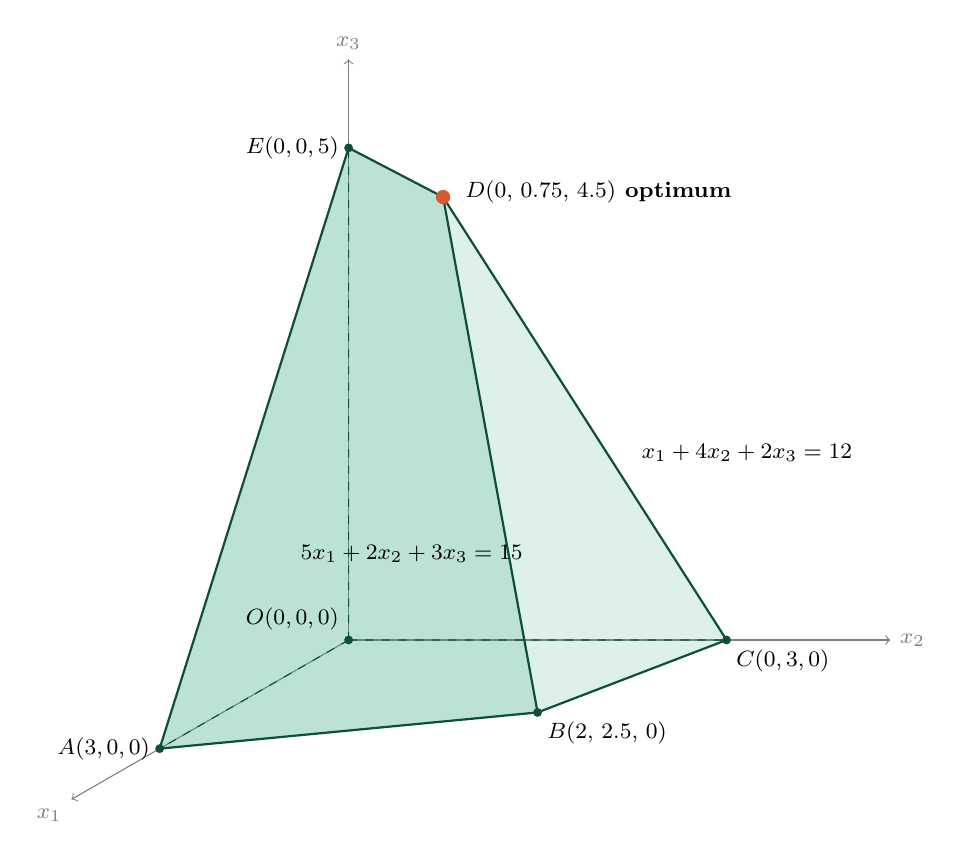
\begin{tikzpicture}[x={(-0.80cm,-0.46cm)},y={(1.6cm,0cm)},z={(0cm,1.25cm)},font=\footnotesize]
\coordinate (O) at (0,0,0); \coordinate (A) at (3,0,0); \coordinate (B) at (2,2.5,0);
\coordinate (C) at (0,3,0); \coordinate (D) at (0,0.75,4.5); \coordinate (E) at (0,0,5);
\draw[->,gray] (O)--(4.4,0,0) node[below left]{$x_1$};
\draw[->,gray] (O)--(0,4.3,0) node[right]{$x_2$};
\draw[->,gray] (O)--(0,0,5.9) node[above]{$x_3$};
\fill[feas,opacity=0.30] (A)--(B)--(D)--(E)--cycle;
\fill[feas,opacity=0.15] (B)--(C)--(D)--cycle;
\draw[dashed,feas!50!black] (O)--(A) (O)--(C) (O)--(E);
\draw[thick,feas!50!black] (A)--(B)--(C)--(D)--(E)--(A) (B)--(D);
\foreach \p in {O,A,B,C,E} \fill[feas!50!black] (\p) circle (1.6pt);
\fill[objc] (D) circle (2.6pt);
\node[above left] at (O) {$O(0,0,0)$};
\node[left] at (A) {$A(3,0,0)$};
\node[below right] at (B) {$B(2,\,2.5,\,0)$};
\node[below right] at (C) {$C(0,3,0)$};
\node[right,font=\footnotesize\bfseries] at ($(D)+(0,0.1,0.05)$) {$D(0,\,0.75,\,4.5)$ optimum};
\node[left] at (E) {$E(0,0,5)$};
\node at (1.7,1.35,1.5) {$5x_1+2x_2+3x_3=15$};
\node[right] at (0,2.25,1.9) {$x_1+4x_2+2x_3=12$};
\end{tikzpicture}
\caption{Problem 4: feasible polyhedron $OABCDE$. The two shaded faces lie on the first two constraint planes.}
\end{figure}

\begin{center}\renewcommand{\arraystretch}{1.2}
\begin{tabular}{clc}
\toprule
Vertex & $(x_1,\,x_2,\,x_3)$ & $f=x_1+2x_2+2x_3$\\
\midrule
$O$ & $(0,\,0,\,0)$ & $0$\\
$A$ & $(3,\,0,\,0)$ & $3$\\
$B$ & $(2,\,2.5,\,0)$ & $7$\\
$C$ & $(0,\,3,\,0)$ & $6$\\
$E$ & $(0,\,0,\,5)$ & $10$\\
\rowcolor{pivot}$D$ & $(0,\,0.75,\,4.5)$ & $\mathbf{10.5}$\\
\bottomrule
\end{tabular}\end{center}
The third constraint $2x_1+x_3\le 8$ is redundant: it is satisfied with strict inequality at every vertex (e.g.\ $x_6=3.5$ at $D$), so it does not form a face of the region. The maximum is at $D$, in agreement with the simplex result.

\subsection*{(c) Python LP solver}
\begin{lstlisting}[language=Python]
"""
MATH 303 - Linear and Nonlinear Programming
Problem 4

    Max  f = x1 + 2 x2 + 2 x3
    s.t. 5x1 + 2x2 + 3x3 <= 15
          x1 + 4x2 + 2x3 <= 12
         2x1       +  x3 <= 8
         x1, x2, x3 >= 0

linprog only minimizes, so we solve  Min f = -(x1 + 2 x2 + 2 x3).
"""
from scipy.optimize import linprog

c = [-1, -2, -2]                    # Min f = -(x1 + 2x2 + 2x3)
A_ub = [[5, 2, 3],
        [1, 4, 2],
        [2, 0, 1]]
b_ub = [15, 12, 8]
bounds = [(0, None)] * 3

res = linprog(c, A_ub=A_ub, b_ub=b_ub, bounds=bounds, method="highs")

print("Status :", res.message)
for i, v in enumerate(res.x, start=1):
    print(f"x{i} = {v:.4f}")
print(f"Max f = {-res.fun:.4f}")
print("Slacks (x4, x5, x6):", res.slack)
\end{lstlisting}
\begin{lstlisting}[style=out]
Status : Optimization terminated successfully. (HiGHS Status 7: Optimal)
x1 = 0.0000
x2 = 0.7500
x3 = 4.5000
Max f = 10.5000
Slacks (x4, x5, x6): [0.  0.  3.5]
\end{lstlisting}

%=====================================================================
\section*{Summary of results}
\begin{center}\renewcommand{\arraystretch}{1.3}
\begin{tabular}{lll}
\toprule
Problem & Optimal solution & Optimal value\\
\midrule
1 & $x_1=62.5,\ x_2=31.25$ & $\max$ profit $=1093.75$\\
2 & $x=6,\ y=0$ & $\max f=6$\\
3 (min) & $x_1=0,\ x_2=5$ & $\min f=20$\\
3 (d, max) & $x_1=4,\ x_2=4$ & $\max f=24$\\
4 & $x_1=0,\ x_2=\tfrac34,\ x_3=\tfrac92$ & $\max f=10.5$\\
\bottomrule
\end{tabular}\end{center}
In every problem the simplex, graphical and Python solutions agree.
\end{document}
